\section{Security of Availability and Validity}


\begin{theorem}[Availability]
Assuming the Merkle tree constructed from collision resistant hash functions and a block in GRANDPA can be finalized with at least $2f+1$ votes, then the availability protocol is secure.
\end{theorem}

\begin{proof}
Assume that an unavailable block is finalized. It means that this finalized block includes a block header of which at most $f$ honest validators has the correct erasure code piece (See Definition \ref{def:unavail}). If this block is finalized, it means that
\begin{itemize}
    \item either not all honest validator who does not have the erasure code piece announce the unavailability. If they would announce it, since their number is at least $2f+1 - f =f+1$ (i.e., honest parties - honest parties who do not have the erasure code), the other honest parties do not finalize it and malicious parties do not have enough number to finalize it. Therefore, we can assume that there is at least one honest party who do not announce the unavailability of its erasure code in this case, because he thinks that he has one but actually it is not correct. If there exists a one honest party who has incorrect erasure code, but having the proof that it is correct (provided by parachain validators), then it means that the collision resistance assumption of Merkle tree is broken. 
    
    \item or  $f+1$ parties announces unavailability it means that GRANDPA finalize the block with at most $2f$  parties. So, this implies that the security of GRANDPA is broken by finalizing a block with less than $2f+1$ votes.
\end{itemize}

Since the GRANDPA is secure and the Merkle tree is collision resistant, the unavailability protocol is secure.
\end{proof}

\begin{theorem}[Validity]
\label{thm:valid}
Assuming that the availability protocol is secure, the signature scheme is EF-CMA secure, the hash function $H$ in Conditions (\ref{cond:time}) and  (\ref{cond:equiv}) is a random oracle, the PoV protocol is secure and correct (Definition \ref{def:pob}), the VRF is secure and a block in GRANDPA can be finalized with at least $2f+1$ votes then the invalid block is finalized in the relay chain with probability less than risk probability.
\end{theorem}

\begin{proof}(Sketch)
TODO: Security reduction, Rewrite the security arguments


If there is one honest $PV$ and there is not any $f+1$ unavailability report, then at least $2f$ of the honest parties has the piece. It means that $PV$ can collect all the pieces from the honest parties in order to reconstruct the blob and check its validity. Therefore, if there is at least one honest party in $PV$, it can detect the invalidity and announces it. In the end, we will have more than $f$ invalidity signatures since the other parties also check invalidity after seeing the signature saying that the block is invalid.

Therefore, we analyze the case where all parachain validators are malicious. 
If there is at least one honest validators who is assigned for extra validity check then the same case happens as having at least one honest parachain validators. Therefore, we need to find out the probability of having all parachain and extra-check validators are malicious given that all parachain validators are malicious. 

There are three cases that the extra check validators are selected: Either with only condition (\ref{cond:mod}) or with condition (\ref{cond:mod}) and (\ref{cond:time}) or with condition (\ref{cond:equiv}). Let's analyze the success of malicious validators in these three cases. Below, $\mu' = \mu+\lceil \runav + \rinv \rceil $ which is the required number of non-parachain validator validity check and $f' < n/3 - n/m$ is the number of non-parachain malicious validators and  $|PV| = n/m = nc$ where $c 1/n$. 

$$\pr[\text{Cond. (\ref{cond:mod})}] =\pr[\text{Cond. (\ref{cond:modequiv})}] = p_{vrf} = \frac{1}{m}$$
$$\pr[\text{Cond. (\ref{cond:time}) at time } \tau] = p_\tau =  \frac{\mu'}{n - nc} + \tau $$
$$\pr[\text{Cond. (\ref{cond:equiv}) }] = \frac{\mu'}{n - nc} $$


%Remark that  with condition (\ref{cond:mod}), we can guarantee that there will be $n/m$ extra validator check. Therefore, if $n/m$ malicious validators do not satisfy the condition (\ref{cond:mod}), then their invalid block is always caught because it means there is at least one honest validator satisfying the condition (\ref{cond:mod}). Therefore, the attacks below are executed when $n/m$ malicious validators satisfy the condition (\ref{cond:mod}). 
\begin{enumerate}


    \item The malicious validators generate an invalid block when they see that at least $\mu'$ malicious validators satisfy the condition (\ref{cond:mod}). This can happen with probability
    
    \begin{equation}\label{eq:attack1cond}
        \sum_{i = \mu'}^{f'}\binom{f'}{i}\frac{1}{m^{i}}(1-\frac{1}{m})^{f'-i}    
    \end{equation}
     which is not negligible. When this happens, their attack succeeds if no honest validator satisfies the condition (\ref{cond:mod}). Then, the attack probability is the following:
	
	\begin{align}\label{eq:nocond1}
	\pr[\mathsf{attack1}] &= \pr[\text{no honest satisfies (\ref{cond:mod})}] \\ \nonumber
									 & \leq   (1-\frac{1}{m})^{2n/3} \\ \nonumber
									 & \leq  e^{-2n/3m} 
	\end{align}
	
	
% 	\item If $\mu' \leq n/m$, the malicious validators generates an invalid block and their attack succeeds since 
	
% 	\begin{align}\label{eq:nocond1}
% 	\pr[\mathsf{attack1}] &=  \binom{f'}{n/m}\frac{1}{m^{n/m}} 
% 	\end{align}

	
    \item The malicious validators generate an invalid block. In this case their attack succeeds if no honest validator satisfies the condition (\ref{cond:mod}) and the condition \ref{cond:time} until a time where at least $\mu'$ malicious validators satisfy the condition \ref{cond:time}. 
    For simplicity, we divide time in discrete values $[\tau_0 = 0, \tau_1 =u, \tau_2 = 2u, ..., \tau_k = ku]$. $\tau_k$ can be computed by malicious validators before the validation process begins. In any case, the only way not to be caught is not to have any honest extra-check validator until $ku$. The probability of this attack is the following:
    
    
    
    \begin{align}\label{eq:attack2}
        \pr[\mathsf{attack2}] &= \pr[\mathsf{attack1}]\prod_{i = 0}^k(1-p_{\tau_i})^{2f+1} \nonumber \\
        &\leq  e^{-2n/3m} \prod_{i = 0}^k (1 - \frac{\mu'+\tau_in(1-c)}{n(1-c)})^{\frac{2n}{3}} \nonumber\\
        &=  e^{-2n/3m} \exp(\sum_{i = 0}^k -\frac{2}{3}\frac{\mu' + \tau_in(1-c)}{1-c}) \nonumber\\
        & = \exp(-2/3(\frac{n}{m}+\frac{(k+1)\mu'}{1-m/n}+ nu\frac{k(k+1)}{2})
    \end{align}
    
    
    % \begin{align}
    %     \pr[\mathsf{attack 2}] \leq \pr[\mathsf{attack }1]\nonumber
				% 						  & = \frac{e^{-2c/3}}{m^{\mu'}} \prod_{i}^k(1-(\frac{\mu'}{n - nc} + \tau_i ))^{2n/3} \leq (1-p_{\tau_0})^{2f+1}\\ &\leq (1-\frac{1+c'_f}{n(1-c)}) ^{\frac{2}{3}n} \nonumber \\
    %     & \leq e^{-2/3\frac{1+c_f}{1-c}} \nonumber
    % \end{align}
    
    
    \item In this attack, the adversary equivocates the block. Here, we can assume that the adversary knows who satisfies the condition (\ref{cond:mod}) since if the malicious validator is the block producer, he first produces the block and sees who validates this block. If no honest validator checks it with condition (\ref{cond:mod}), he equivocates it.  We know that probability of no honest party satisfies the condition (\ref{cond:mod}) is given in  inequality (\ref{eq:nocond1}). When this happens, the attack succeeds if no honest party satisfies the condition (\ref{cond:modequiv}) and (\ref{cond:equiv}). 
    The probability of attack 3 is
    
    \begin{align}
    \pr[\mathsf{attack} 3] &=\pr[\text{no honest check in  cond. (\ref{cond:equiv}) and (\ref{cond:modequiv})}]\nonumber \\ 
							&\leq \pr[\mathsf{attack1}](1-\frac{\mu'}{n-nc)}) ^{\frac{2}{3}n} \nonumber\\
				            & \leq \exp({-2/3(\frac{n}{m}+\frac{\mu'}{1-m/n})}) \nonumber
    \end{align}
\end{enumerate}	
    % \item  In this attack, the adversary equivocates and it does it when $\mu'> n/m$ and there are $n/m$ malicious adversaries satisfying the condition (\ref{cond:mod}). we can assume that the adversary knows who satisfies the condition (\ref{cond:mod}) since if the malicious validator is the block producer, he first produces the block and sees who validates this block. If no honest validator checks it, he equivocates it with a block where at least $n/m$ malicious validators satisfies the condition (\ref{cond:modequiv}). Then, the attack succeeds if no honest party satisfies the condition (\ref{cond:equiv}). 
    % The probability of attack 3 is
    
    % \begin{align}
    % \pr[\mathsf{attack}3] &=\pr[\text{no honest check in  cond. (\ref{cond:equiv})}]\nonumber \\ 
				% 					   &\leq (1-\frac{\mu'}{n-nc)}) ^{\frac{2}{3}n} \nonumber\\
				% 					   &\leq e^{-2/3(\frac{\mu'}{1-c})} \nonumber
    % \end{align}
    
    





%
%Therefore, the attack probability is $\pr[\mathsf{attack1}]+\pr[\mathsf{attack2}]+\pr[\mathsf{attack}3]$.



%Here, we consider $r_a = 0$ to compute the maximum attack probability and $c_f' = \lceil r_f \rceil$. We do not take $r_f = 0$, because we assume that there is always at least one fisherman.


%a parachain validator does not know who are the extra-check validators except the malicious validators if they are assigned to extra check. This comes from the VRF security. So , since $H$ is a random oracle, $B$ is derived from a uniform distribution between $[0,1]$. Therefore, the probability of a validator is assigned to be an investigator at time $\tau$ given that not enough validity check (i.e., $|\mathcal{I}| < \vcheck$) is done before $\tau$ is:

%$$p_{\tau} = \frac{\vcheck - |\pv|}{|\V|-|\pv|}+\tau  = \frac{1+\lceil \runav + \rinv \rceil}{n-nc}+ \tau$$

%assuming that $|PV| = nc$ where $c \in (0,1)$.

%Remark that when $\tau$ increases meaning that when the time increases without having sufficient validity check, $p_{\tau}$ increases and reaches 1 at some time. For simplicity, we divide time in discrete values $[\tau_0 = 0, \tau_1 =\mu', \tau_2 = 2\mu', ..., \tau_k = k\mu']$ where $k\mu'$ is the time when the number of malicious parties in $\mathcal{I}$ is $\vcheck$. This time can be computed by malicious validators before the validation process begins. In any case, the only way not to be caught is not to have any honest extra-check validator until $k\mu'$. The probability of this is the following given that  the number of malicious parties in $\mathcal{I}$ is $\vcheck$:

%\begin{align}
% \pr[\mathsf{attack} = 1] = \prod_{i = 0}^k(1-p_{\tau_i})^{2f+1} \leq (1-p_{\tau_0})^{2f+1} &\leq (1-\frac{1+c'_f}{n(1-c)}) ^{\frac{2}{3}n} \nonumber \\
%& \leq e^{-2/3\frac{1+c_f}{1-c}} \nonumber
%\end{align}
%Here, we consider $r_a = 0$ to compute the maximum attack probability and $c_f' = \lceil r_f \rceil$. We do not take $r_f = 0$, because we assume that there is always at least one fisherman.



\end{proof}


%As result, $e^{-2/3\frac{1+c_f}{1-c}}$ needs to small enough so that the malicious validator do not consider to risk their stake.

\subsection{Parameter Selection}

Remark that all the attacks in the proof of Theorem \ref{thm:valid} can succeed if all parachain validators are malicious and this happens with the probability $\frac{1}{3^{n/m}}$.


All attacks above depend on two parameters, $\mu$ and $n/m$. Therefore, we need to specify these parameters so that the attack probabilities are less than the risk probability. The risk probability is critical here and we should find a way to define it. Informally, the risk function is defined as follows: When the certain conditions are satisfied to execute attack 1, attack 2 or attack 3, whatever the adversary gain when he executes the attack needs to be smaller than whatever he loses when the attack is unsuccessful. 

\begin{equation}
    \pr[\mathsf{attack X}]\mathsf{Gain} < (1-\pr[\mathsf{attack X}])\mathsf{Lost}
\end{equation}

We can assume that $\mathsf{Gain}$ at most equals to all stake of validators (I am not sure how logical to define it like this ) and $\mathsf{Lost}$ equals to stake of parachain validators. In this case, we obtain

\begin{equation}\label{eq:attackgain}
    \frac{\pr[\mathsf{attack X}]}{1-\pr[\mathsf{attack X}]} < \frac{sn/m}{sn} = \frac{1}{m}
\end{equation}

\paragraph{The relation between $n$ and $m$:} When we compare the probability of attacks, clearly, attack 1 is more probable than the others. Therefore, we need to make sure that probability of attack 1 satisfies the relation in (\ref{eq:attackgain}). In order to have this relation, we should have the following inequality between $n$ and $m$:

\begin{equation}\label{eq:relation}
    n > \frac{3m\ln(m+1)}{2}
\end{equation}

\paragraph{Selection of $\mu$:} Since attack 1 is the most probable attack, we also need to make sure that the necessary condition to execute attack 1 should happen very rarely. Remember that the necessary condition to execute the attack 1 is having at least $\mu$ malicious validators in condition (\ref{cond:mod}).  To bound this probability, we consider the case when all parachain validators are malicious which can happen with probability $\frac{1}{3^{n/m}}$. Assuming that the set of parachain validators changes in each epoch, the probability of satisfying the necessary condition in one slot to execute attack 1 (Equation (\ref{eq:att1cond})) should be less than $\frac{1}{\zeta}$ where $\zeta$ is the expected number of malicious slots in one epoch. 
\begin{equation}\label{eq:att1cond}
    p'_1 = \pr[\text{at least }\mu \text{ malicious in cond. (\ref{cond:mod})}] = \sum_{i = \mu}^{f'}\binom{f'}{i}\frac{1}{m^i}(1-\frac{1}{m})^{f'-i}
\end{equation}
According to  \href{http://research.web3.foundation/en/latest/polkadot/BABE/Babe/#6-practical-results}{BABE practical results} (e.g., $c = 0.034, T = 3$ and $k = 54$ ), the epoch length should be around 20000 slots and expected number of malicious slots are around 215. With this constraint, we need to have the parameter $\mu$ as shown in Figure \ref{fig:muval} with respect to $m$.  

\begin{figure}[h]\centering
	  \includegraphics[width=16cm]{images/muval.png}
	  \caption{The parameter $\mu$ according to number of parachains}
	  \label{fig:muval}
\end{figure}

Now, let's analyze attack 2 and attack 3 with the parameterization above.

Actually, there is not any condition for attack 2 which means that it can be executed in any block. The reason of this is that there exists always a $k \in \mathbb{N}$ which let at least $\mu$ malicious validators being selected for the extra check in every block. When the adversary executes the attack 2, we assume that $x < \mu$ malicious validators satisfy the condition (\ref{cond:mod}) and at least $\mu - x$ malicious validator satisfy the condition (\ref{cond:time}) until the time $\tau_k$. The best case for the adversary in order to have the highest probability in attack 2 (See (\ref{eq:attack2})) is when $k = 0$. Therefore, the best case probability is the following:

\begin{align}\label{eq:att2cond}
    p'_2 &= \sum_{x=0}^{\mu-1}\pr[\text{x malicious is in cond. (\ref{cond:mod})}]\pr[\text{at least }\mu-x\text{ malicious in cond (\ref{cond:time}) when } k = 0] \nonumber \\
    &= \sum_x^{\mu-1}\binom{f'}{x}\frac{1}{m^{x}}(1-\frac{1}{m})^{f'-x}\sum_{i = \mu-x}^{f'}(\frac{\mu}{n-n/m})^{i}(1-\frac{\mu}{n-n/m})^{f'-i}
\end{align} 

We can see that with the selection of the parameter $\mu$ according to $p'_1$ in Equation (\ref{eq:att1cond}), $p'_2 > 1/\zeta$. This means that the malicious parties will have more chance to be in the best case in one epoch. However, since the probability of attack 2 is very low considering the gain/lost relation, any rational malicious validator do not execute the attack 2.


Lastly, we analyze attack 3. The  condition for attack 3 is to have no honest validator satisfying the condition (\ref{cond:mod}) which can happen with the probability

\begin{equation}\label{eq:att3cond}
    p'_3 = \pr[\text{no honest in condition (\ref{cond:mod})}] = (1-\frac{1}{m})^{2n/3}.
\end{equation}
In the analysis of attack1, we fix this probability to almost $1/m$. Similar to attack 2, if $m < \zeta$, then parachain validators are malicious, they have more chance to execute the attack 3 during their period. With the same probability as in attack 2, executing attack 3 is too risky for the adversary considering its gain and lost.

The claim that any rational adversary doe not execute attack 2 or attack 3 can be clearly seen in the  Figure \ref{fig:attack123}.

\begin{figure}[h]\centering
	  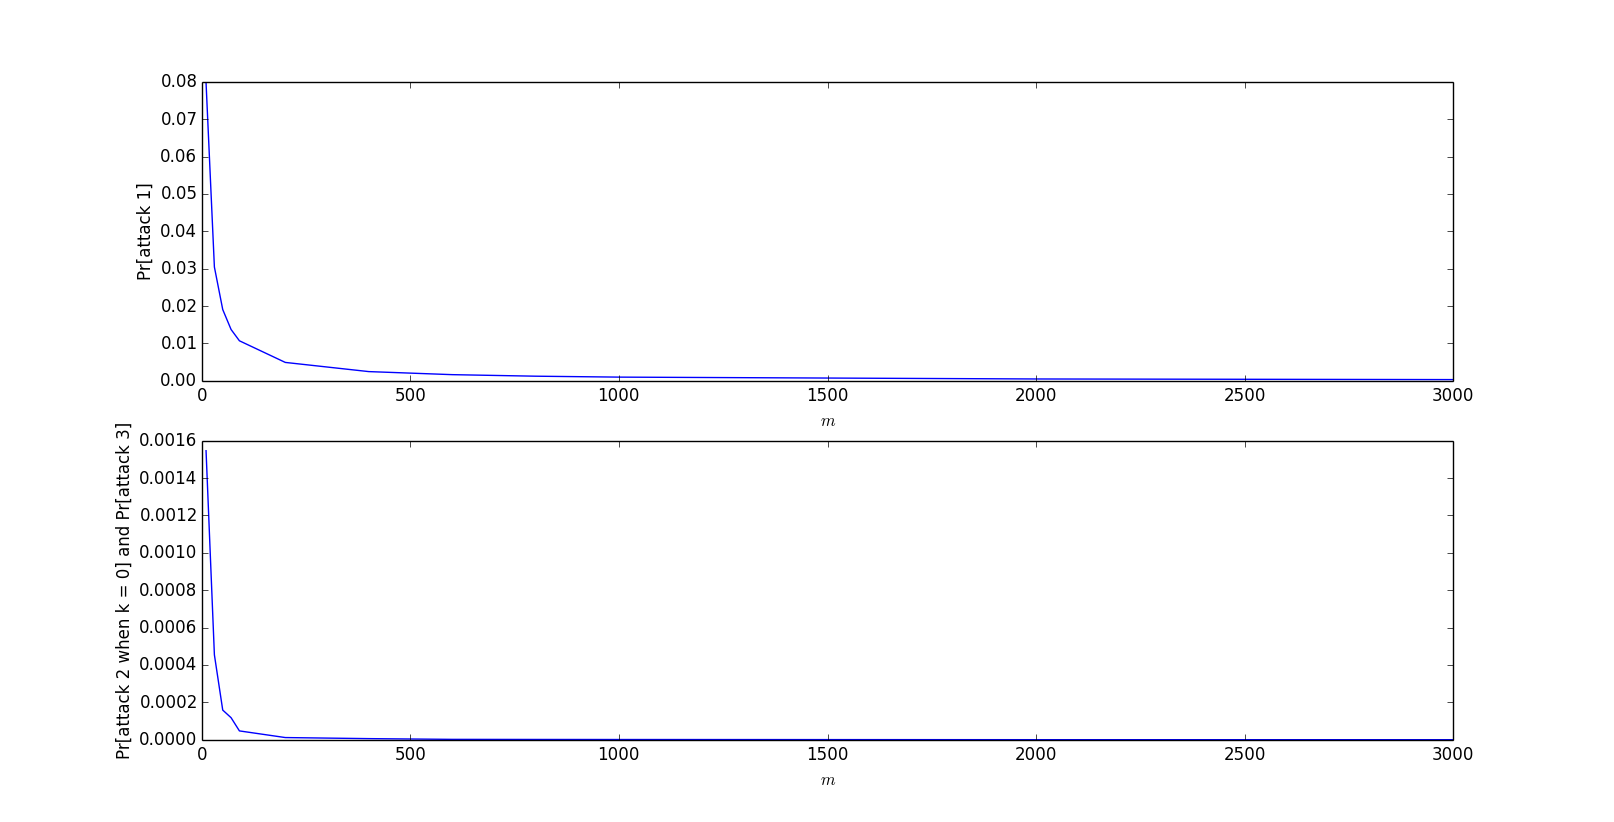
\includegraphics[width=16cm]{images/attack123.png}
	  \caption{The success probabilities of attack 1, 2 and 3}
	  \label{fig:attack123}
\end{figure}


We give the total attack probabilities (i.e., $p'_X\pr[\mathsf{attack X}]$)is given in the Figure \ref{fig:total}. As it can be seen the success of the attacks are very low. Remember that all these attacks can be happen when all parachain validators are malicious. So, in this case, they have this probability. Otherwise their success probabilities are 0.

\begin{figure}[h]\centering
	  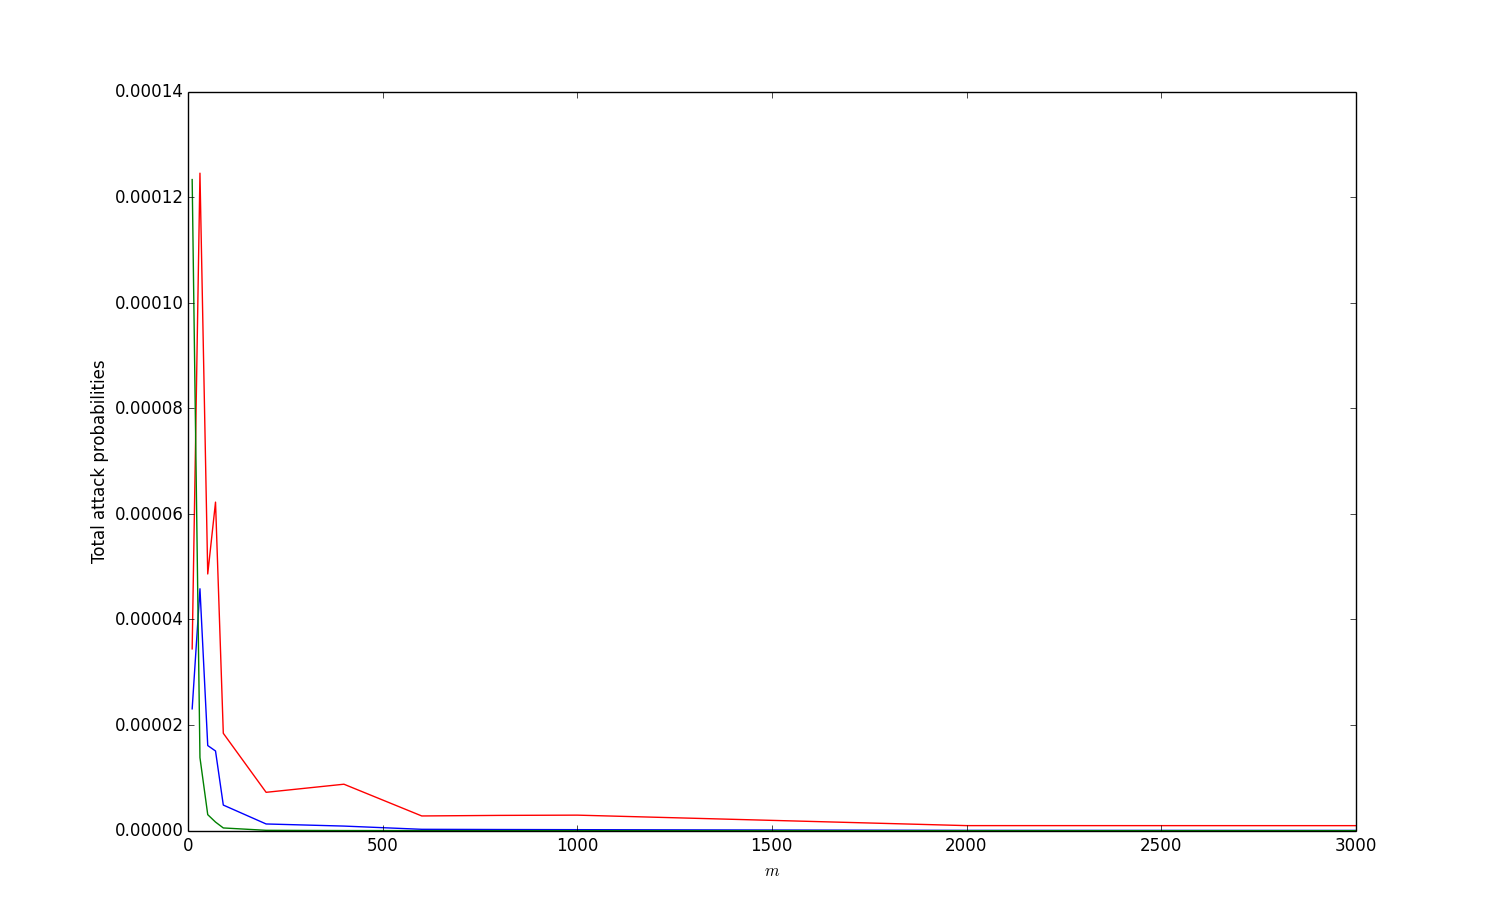
\includegraphics[width=16cm]{images/totalattack.png}
	  \caption{The total attack probabilities. Red is for attack 1, blue is for attack 2 and green is for attack 3.}
	  \label{fig:total}
\end{figure}




% We first compare the conditions to execute the attack 1, attack 2 and attack 3. The condition for attack1 is to have at least $\mu$ malicious validators satisfying the the condition (\ref{cond:mod}) which is given in the probability below:






% The attack 3 condition is to have no honest validator satisfying the condition (\ref{cond:mod}) and it probability is:

% \begin{equation}\label{eq:att3cond}
%     p'_3 = \pr[\text{no honest in condition (\ref{cond:mod})}] = (1-\frac{1}{m})^{2n/3}
% \end{equation}


% When we compare $p'_1, p'_2$ and $p'_3$ (See equations (\ref{eq:att1cond}), (\ref{eq:att2cond}) and (\ref{eq:att3cond}), respectively), we see that $p'_2$ is the greater than the others. Therefore, we choose the parameter $\mu$ according to $p'_2$ to make $p'_2$ is very small so $p'_1$ and $p'_3$ too. 

% First, let's analyze the probability of attack 1 which depends only $n/m$ to find a relation between $n$ and $m$ with using equation \ref{eq:attackgain}. Then, we obtain

% \begin{equation}\label{eq:relation}
%     n > \frac{3m\ln(m+1)}{2}
% \end{equation}

% If we preserve this relation then the attack 1 (and so attack 2 and attack 3) will be small enough so that the adversarial gain from this attack is small comparing to his lost.

% Now, consider the case where all parachain validators are malicious and assume that the set of parachain validators changes in each epoch. In this case, the probability of satisfying the necessary condition in one slot to execute attack 1 should be less than $\frac{1}{\zeta}$ where $\zeta$ is the expected number of malicious slots in one epoch. According to  \href{http://research.web3.foundation/en/latest/polkadot/BABE/Babe/#6-practical-results}{BABE practical results} (e.g., $c = 0.034, T = 3$ and $k = 54$ ), the epoch length should be around 20000 slots and expected number of malicious slots are around 215.  


% \begin{figure}[h]\label{fig:muval}\centering
% 	  \includegraphics[width=8cm]{muval.png}
% 	  \caption{The parameter $\mu$ according to number of parachains}
% \end{figure}


% Analysis of attack 2 is different than attack 1 because for this attack, the adversary do not need to wait for satisfying a specific condition (e.g., for attack 1, the adversary should wait for the block where at least $\mu$ malicious validators satisfy the condition (\ref{cond:mod})). The reason of this is that there exists always a $k \in \mathbb{N}$ which let at least $\mu$ malicious validators being selected for the extra check in every block. When the adversary executes the attack 2, we assume that $x < \mu$ malicious validators satisfy the condition (\ref{cond:mod}) and at least $\mu - x$ malicious validator satisfy the condition (\ref{cond:time}) until the time $\tau_k$. The best case for the adversary in order to have the lowest probability in attack 2 (See (\ref{eq:attack2})) is when $k = 0$. Therefore, the best case probability needs to be less than $1/\zeta$ for all $x$. The best case probability is the following:

% \begin{equation}\label{eq:bestcaseinatt2}
%     \pr[\text{best  case for }\mathsf{attack 2}] = \sum_x^{\mu-1}\binom{f'}{x}\frac{1}{m^{x}}(1-\frac{1}{m})^{f'-x}\sum_{i = \mu-x}^{f'}(\frac{\mu}{n-n/m})^{i}(1-\frac{\mu}{n-n/m})^{f'-i}
% \end{equation}

% If we choose  the parameter $\mu$ as in Figure \ref{fig:muval}, the best case probability will be greater than $1/\zeta$ as it can be seen in Figure \ref{fig:bestforattack2}. It means that when parachain validators are malicious, they have more chance to execute the attack 2 during their period. However, the probability of executing the attack 2 is much smaller than attack 1 probability which less than $1/m$. It means that it is too risky for the adversary to execute attack 2 considering the risk function in Equation (\ref{eq:attackgain}).

% \begin{figure}[h]\label{fig:bestforattack2}\centering
% 	  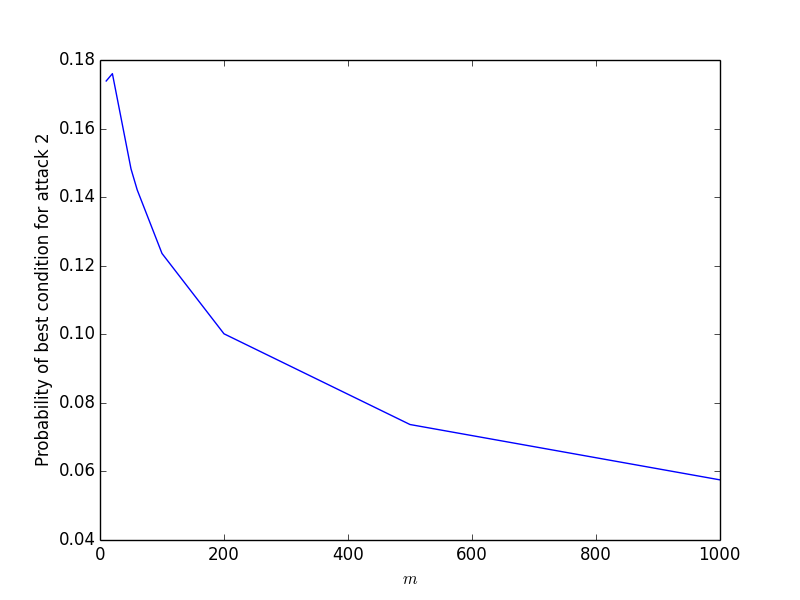
\includegraphics[width=8cm]{bestcond.png}
% 	  \caption{The probability of having the best case for attack 2.}
% \end{figure} 

% Lastly, we analyze attack 3. The attack 3 condition is to have no honest validator satisfying the condition (\ref{cond:mod}). In the analysis of attack1, we fix it to $1/m$. Similar to attack 2, if $m < \zeta$, hen parachain validators are malicious, they have more chance to execute the attack 3 during their period. With the same probability as in attack 2, executing attack 3 is too risky for the adversary considering its gain and lost.

% The total attack probabilities is given in the graph below:

%If the number of parachain increases, we can see that the probability of having all parachain validators malicious decreases. However, the probability of  condition for attack 1 (See equation \ref{eq:attack1cond}) increases when $m$ increases if $\mu$ is constant. Therefore, the parameter $\mu$ needs to be selected according to number of parachains.






% The adversaries satisfies the condition to execute the attack if at least $\mu$ malicious validators are in condition (\ref{cond:mod}). Given a fixed number of parachain, if number of validator increases then the probability in \ref{eq:cond1} increases. On the other hand, the probability of attack1 decreases. Therefore, in this case, we need to find $n/m$ which makes attack 1 probability low enough and according to this find a $\mu$ value which make \ref{eq:cond1} low enough.


% The condition for attack 1 is to have $\mu'$ malicious validators in the condition (\ref{cond:mod}). This condition happens with probability $\binom{f'}{\mu'}\frac{1}{m^{\mu'}} $.
% We do not have any condition for attack 2.
% The condition of attack 3 is that there is no honest party satisfying condition $(\ref{cond:mod})$. This happens with probability $\pr[\mathsf{attack1}] \leq \exp(-\frac{2n}{3m})$.


% So, first of all we need a relation between $n$ and $m$  so that the probability of attack 1 is small enough so that attack 2 and attack 3. Considering the economics of the entire protocol, this probability needs to be smaller than $1/m$. In this case, we have the following relation between $n$ and $m$:

% \begin{equation}\label{eq:nm}
%     n > \frac{-3m\ln(m^{-1})}{2}
% \end{equation}


% In addition, the good conditions for attack 1 needs to be small enough so that the adversaries won't have many chances to execute attack 1.




% There are certain parameters that we need to fix to make sure the security of the protocol. 


% Remark that attack 1 (See inequality (\ref{eq:nocond1})) only depend of number of parachain  validators $n/m$.  As it can be seen in Figure \ref{fig:attack1prob}, if the ratio of number of validators and parachain validators are more than 10, the the attack1 probability is very close to 0. Therefore, it is critical to satisfy this ratio to have security.

% \begin{figure}[h]\label{fig:attack1prob}\centering
% 	  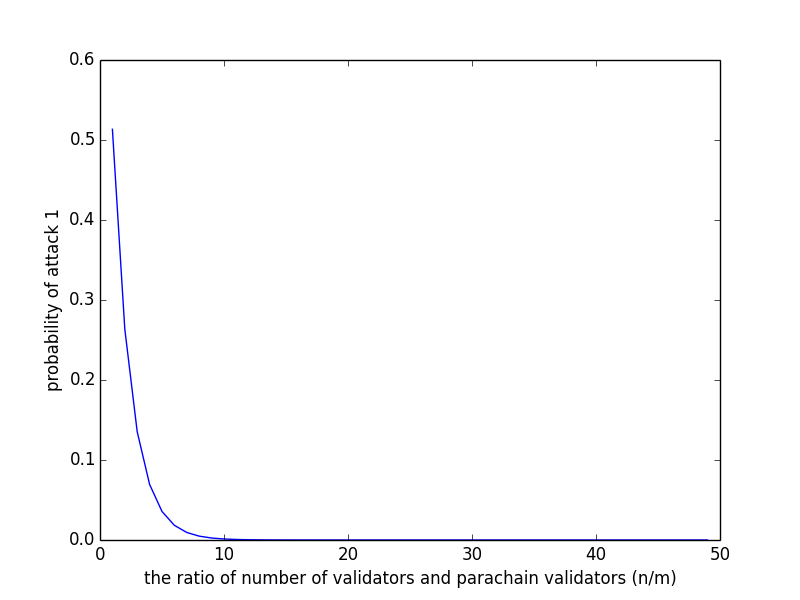
\includegraphics[width=7.5cm]{attack1.png}
% 	  \caption{The probability of attack 1 which depends on $|PV| = n/m$}
% \end{figure}




% In our next analysis for attack 3, we assume that $|PV| = n/m \geq 10$ so $c\geq 10/n$. In our attack 3 analysis, we find the minimum number of extra check $\mu$ for security.
% In the case of all collators are malicious and collaborating with the parachain validators, they prefer to make the blob unavailable to fishermen. Therefore, we cannot rely on fishermen in this case because they will not access the block to check the validity. Besides, we do not receive any unavailability report from collators. Therefore, if all collators are malicious, it makes sense to assume that $\runav + \rinv = 0$, and so $\mu' = \mu$. Even in this case, the above attack probabilities has to be low enough for the malicious parties so that they do not to risk their stake and reputation. In below Figure \ref{fig:attack3prob}, it can be seen that $\mu$ needs to be at least between 8 and 10 in order to have very low attack 3 probability.


% \begin{figure}[h]\label{fig:attack3prob}\centering
% 	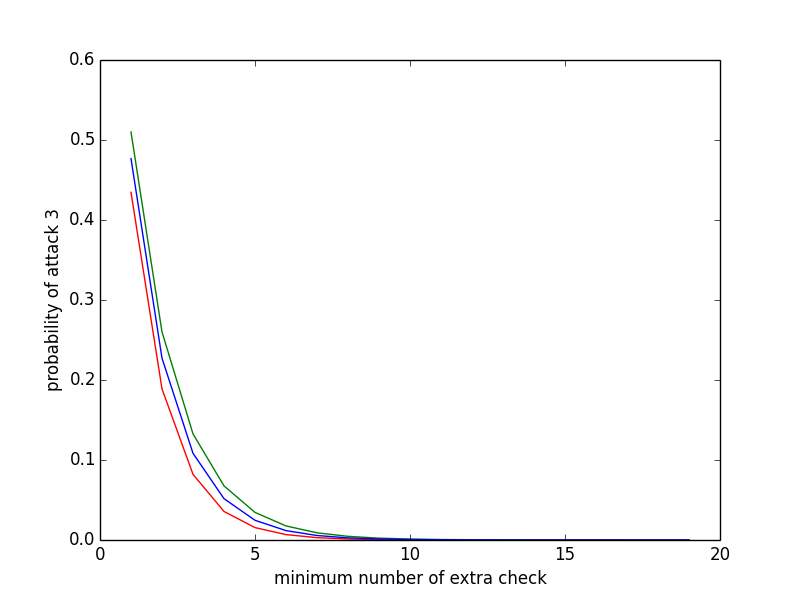
\includegraphics[width=7.5cm]{attack3.png}
% 	\caption{The probability of attack 3 which depends on number of validators and $\mu$. In red graph $n = 50$, in blue graph $n = 100$ and in green graph $n = 1000$.}
% \end{figure}



% In the case where all collators are not malicious, we can rely on the unavailability reports from collators.